\subsection{Sensing Subsystem}
\label{sec:sensing_subsystem}
\begin{figure}[H]
    \caption{Sensing subsystem block diagram}
    \centering
    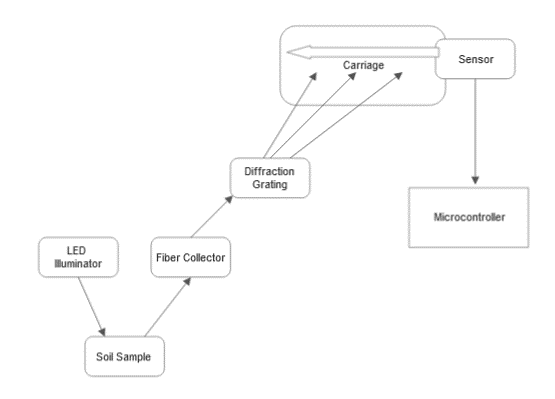
\includegraphics[width=0.75\textwidth]{images/OpticsBlockDiagram.png}
\end{figure}


The sensing subsystem is an infrared spectrometer that uses two photodiodes as detectors, a diffraction grating as a spectral separator, an array of LEDs to illuminate the target area, and optics to collect, collimate, and focus the beam. In order to determine the component positions and interaction, each component will have to be addressed.
    \begin{itemize}
        \item Ground
        \item LEDs
        \item Fiber in
        \item Fiber out collimated
        \item Reflective Diffraction Grating
        \item Focusing Lens
        \item Carriage driven Photodiodes
        \item Filter Circuitry
    \end{itemize}


    \paragraph{Dirt}

That’s right, the first part of the optical subsystem is the soil. Structures in the soil emit trace electromagnetic signals that correspond to the soil matrix, soil temperature, soil moisture, and chemical content of the soil. (Link papers)
In order to ensure sufficient signal to noise ratio, the dirt is going to have to be probed by a bright, broadband source covering the visible and Near Infrared regime. Halogen lamps will do (link papers) but it may be possible to achieve the same effect with LEDs near the surface. 
An additional concern is that irregularities in the soil topography may reflect back light that would otherwise indicate organic components or water. In order to counter this, it is going to be necessary to flatten the dirt with a stamp or roller.


\paragraph{LEDs}

Placeholder until followup with ocean insight.

\paragraph{Fiber in}

placeholder

\paragraph{Fiber out collimated}

The fiber collimator selection hasn’t been finalized yet, but for now I’m assuming a beam of about 2mm diameter will come out of the fiber head collimated toward the grating.

\paragraph{Grating}

    The grating will be a 1200 groove per mm aluminum coating 1000nm blazed reflection grating. 
 
The grating equation governs the angle at which light of different frequencies will reflect. 
The first three orders of diffraction are plotted below for a 1200 groove per mm grating. The polar plot is degrees, ranging from 400nm to 1700nm. Rho represents the order of diffraction.
An angle of incidence of 45 degrees will produce backreflection toward the fiber collimator, however an angle of incidence at 50 degrees will not.



\begin{figure}[H]
    \caption{Diffraction angle calculation}
    \centering
    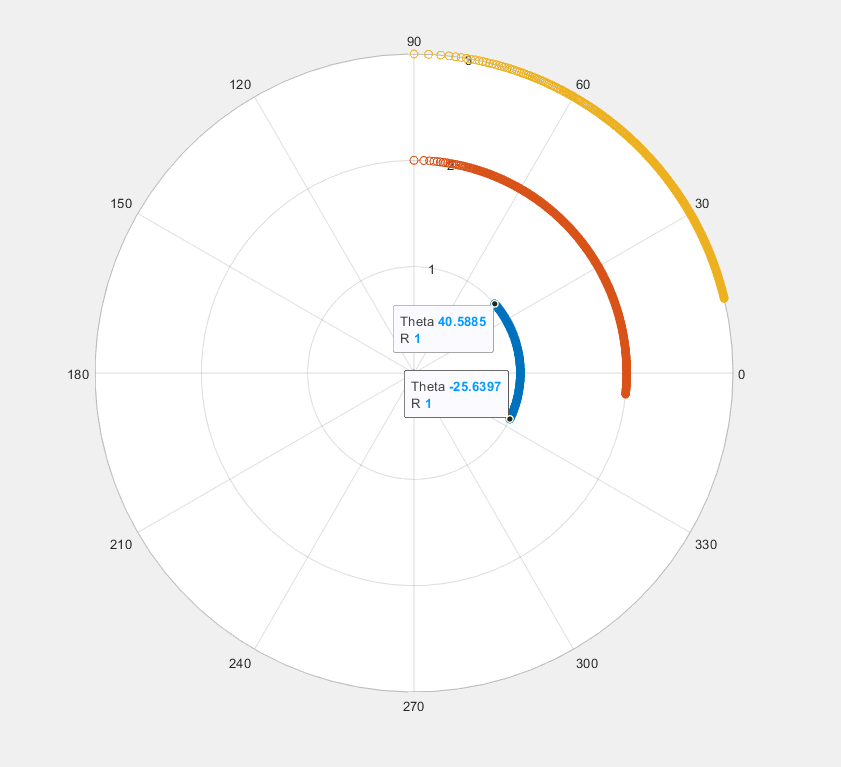
\includegraphics[width=0.75\textwidth]{images/DiffractionAngleCalculator.png}
\end{figure}

\paragraph{Focusing Lens}

\paragraph{Carriage driven Photodiodes}

\begin{figure}[H]
    \caption{Photodiode Signal Filter}
    \centering
    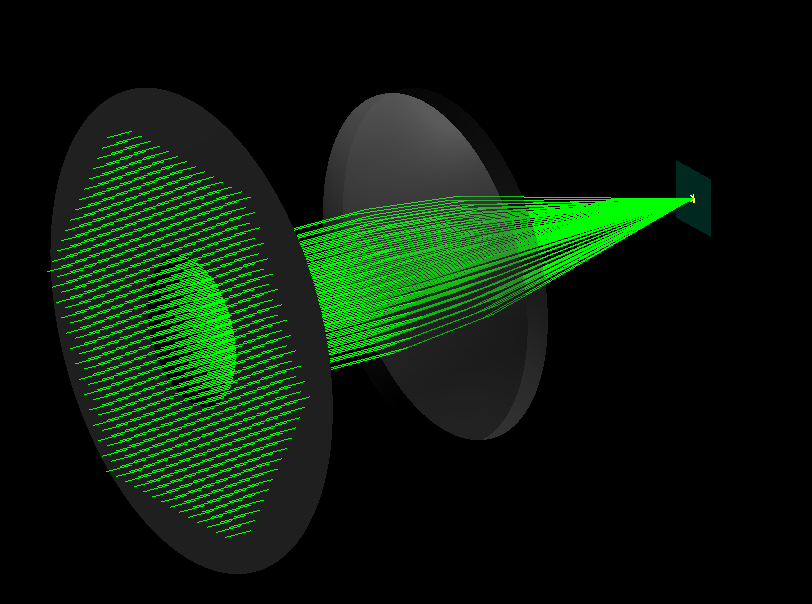
\includegraphics[width=0.75\textwidth]{images/ColimatedBeam.png}
\end{figure}

\paragraph{Signal Filtering}

\begin{figure}[H]
    \caption{Photodiode Signal Filter}
    \centering
    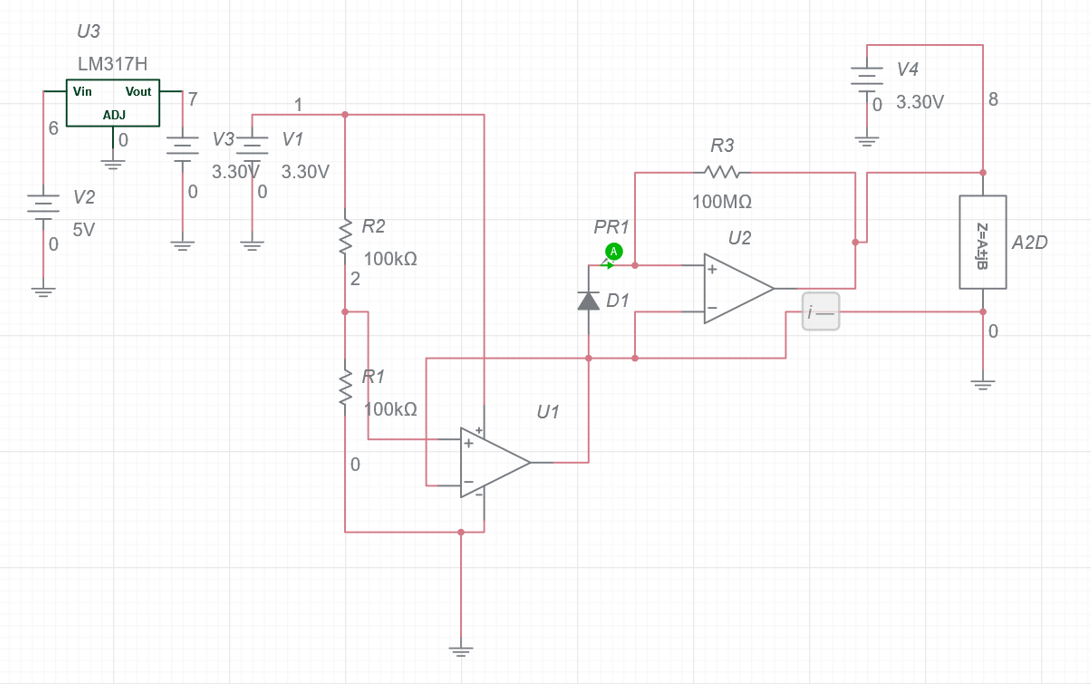
\includegraphics[width=0.75\textwidth]{images/ElectricalSignalFilteringSD1.png}
\end{figure}


The Photodiode works by converting a small portion of the incident light into electrical current across the face of the semiconductor. The diode will have a small current running through the circuit hooked up to an amplifier for boosting the signal to a detectable level. Then another op amp will cut out the electrical noise created by unwanted frequencies generated by the diode and electromagnetic interference.

